\section{Software Design}
\phantomsection
\subsection{UML Modeling}
In the current chapter is represented and described the architecture of OpenMedia application. It contains a set of relevant diagrams modeled in UML language. The diagrams provide a fundamental documentation an description of the system structure and behavior.

The aspect that should be defined is how user will interact with the application. Therefore a use case diagram was modeled to show the set of available actions offered at user's disposal. The client part of the application represents a browser web page. There are five main actions an user can performed. The operations can be seen in \mbox{figure \ref{use_case}}. When the applications is opened, the user can complete the basic word frequency search. The second action asks the application to fulfill trend detection analysis. The user will be able to set the intervals on which the trends disclosure is achieved. The remaining options of interaction with the applications aims to visualize the information on the performed tasks. For instance the action of displaying the word frequency renders the density of a specific word, under the form of a line chart. Trend detection results has an analogical approach of representation, it differentiates by the type of plot.

\begin{figure}[!ht]
\centering
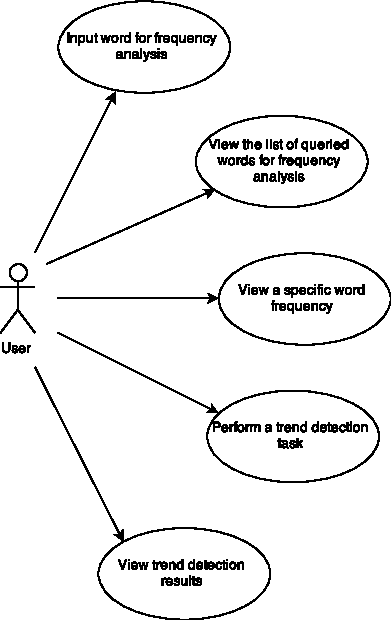
\includegraphics[width=8cm]{2_use_case}
\caption{User use case diagram}\label{use_case}
\end{figure}

To offer a detailed overview of how the entire system works, a set of sequence diagrams are provided. They show key parts of the platform and the way they interact. Moreover it is crucial to depict the depth of chain of events happening in the background. For instance the sequence diagram, shown in \mbox{figure \ref{user_sequence}}, specifies what happens when a user does a simple word frequency query. First of all the client browser does an HTTP request in order to get the application page. Now the user is able to interact with OpenMedia platform. When the client requests a word frequency, two events are fired. First is an AJAX request that aims to launch the task. The second thing is subscribing to a websocket channel that allows to receive the task finished notification. The web application launches an asynchronous job on the Sidekiq server. When the job has finished, it sends an HTTP request to the websocket server. The next and the last thing is that client's web page receives the notification because it was subscribed to the channel.

\begin{figure}[!ht]
\centering
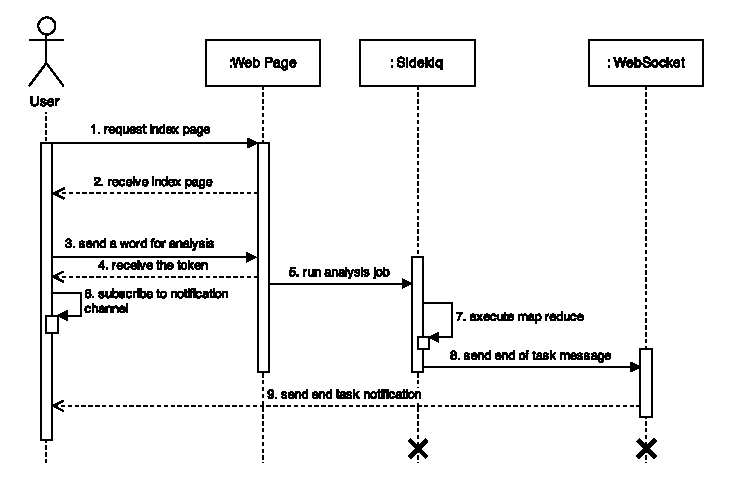
\includegraphics[width=15cm]{2_user_sequence}
\caption{User Sequence Diagram}\label{user_sequence}
\end{figure}

The client application is only one part of OpenMedia. The data gathering side consists of three main steps. Each one is described in the sequence diagrams illustrated below. Their behavior looks similar, nevertheless each has unique characteristics worth pointing out.

First step of data gathering process is fetching the articles, that is depicted in \mbox{figure \ref{fetcher_sequence}}. The entry point of the application is a makefile that runs ruby scripts. Every media source has a custom fetcher class, nevertheless they all posses the same interface. The main script instantiates every type of fetcher and runs it. The articles retrieving class is smart enough to be able get the all the accessible articles in an iterative way, followed by saving the data on the files storage. The entire process is straight and monotonous. The preconditions are, for public media provider's servers to be up and running and as for the local machines it is required to be connected to an ISP provider.

\begin{figure}[!ht]
\centering
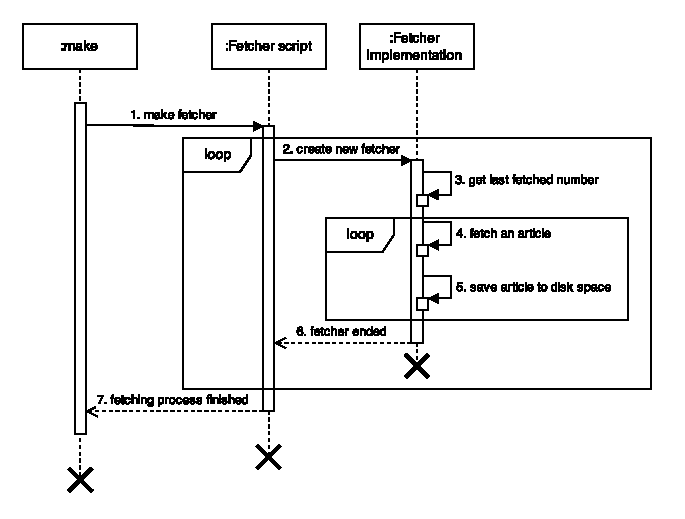
\includegraphics[width=15cm]{2_fetcher_sequence}
\caption{Article fetcher sequence diagram}\label{fetcher_sequence}
\end{figure}

The sequence diagram, illustrated in \mbox{figure \ref{parser_sequence}}, represents the action of parsing the fetched articles. It is the second step in the data gathering cycle. It works analogically as the first part. Due to the fact that every media source has their own way to represent the article concludes that each source should have a custom parser. But again with a similar interface. The parsing script instantiates a custom parser object and runs it. The custom object is able to retrieve the fetched articles from the file storage, extract the meaningful information and save it back to a database. This action is represented on the diagram in a iterative way.

\begin{figure}[!ht]
\centering
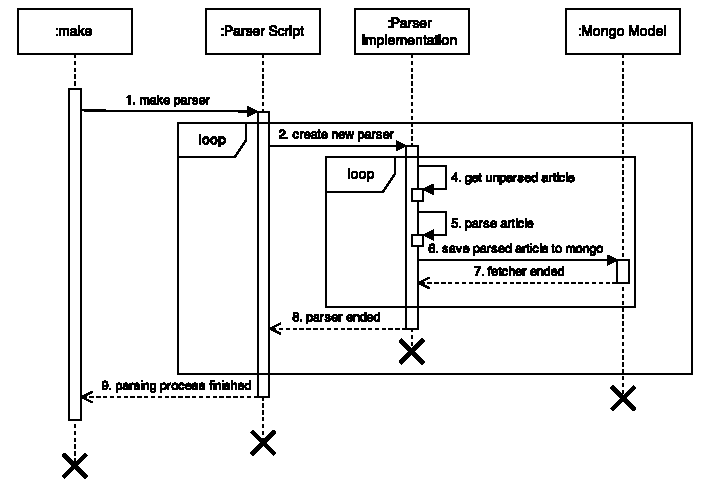
\includegraphics[width=15cm]{2_parser_sequence}
\caption{Article parser sequence diagram}\label{parser_sequence}
\end{figure}

The last, time consuming, step in the data mining cycle is executing natural language processing on the given data. In context of OpenMedia this part is decisive. Running analysis on simple chunks of text is inefficient. Which is why text should be annotated with metadata such as part of speech, lemmatized forms etc. The way it differs from the previous steps is that it does not need customized classes. Presumably the articles are already saved under the same form, the scripts iteratively extracts articles. Each iteration undergoes a sequence of NLP operations, that can be observed in the diagram \mbox{figure \ref{nlp_sequence}}. The operations are: tokenization, part of speech tagging etc. The last step of an iteration is splitting the articles and saving back to database under a different form.

\begin{figure}[!ht]
\centering
\vspace*{0.6cm}
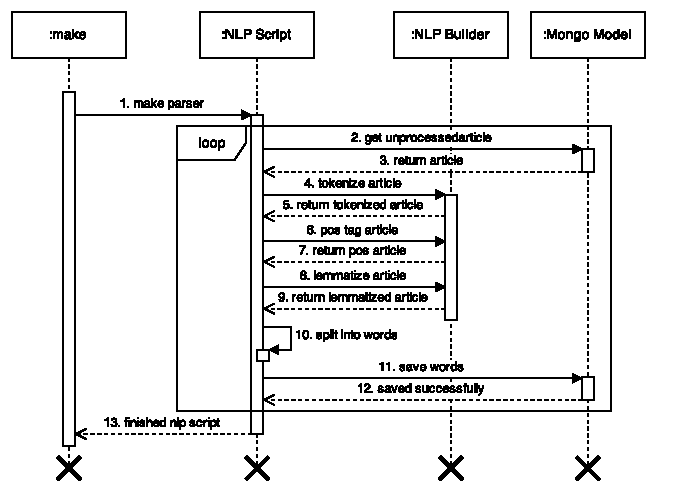
\includegraphics[width=15cm]{2_nlp_sequence}
\caption{NLP script sequence diagram}\label{nlp_sequence}
\end{figure}

Until now every step of data mining process was described particularly. On an abstract level, the activity diagram, illustrated in figure \mbox{\ref{data_mining_activity}}, represents the sequence of actions performed on the data gathering part of the application. Every executed step depends on the previous one. There is also the final part, that was not mentioned in the sequence diagrams. This part performs a series of tasks which preprocess the tokenized data. The resulted data is optimized for frequency analysis tasks. More details will be provided in the implementation chapter of the report.

\begin{figure}[!ht]
\centering
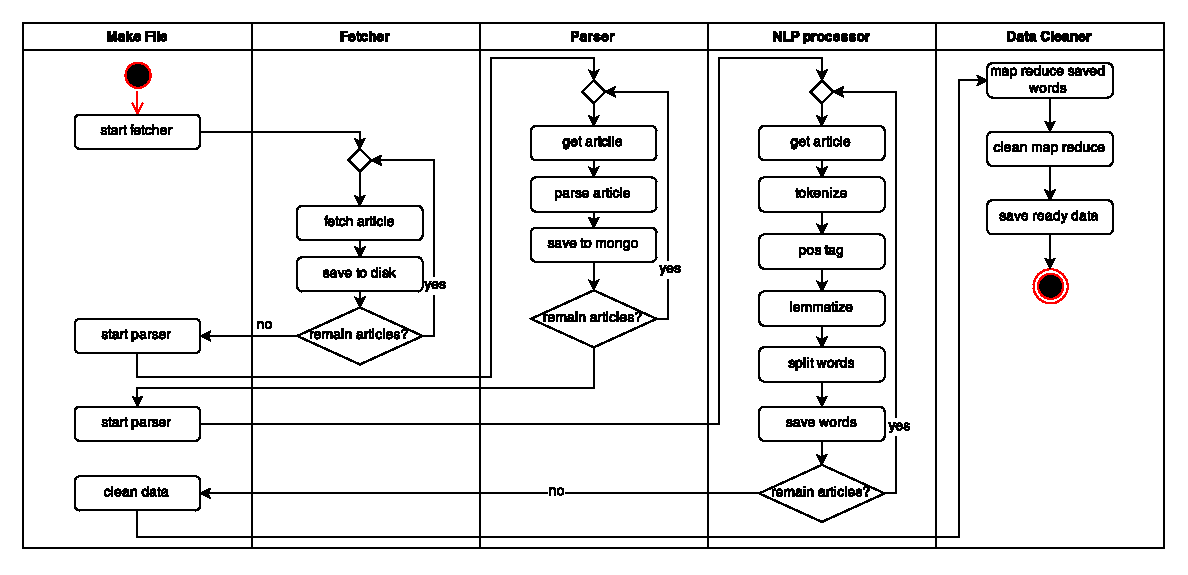
\includegraphics[width=18cm]{2_data_mining_activity}
\caption{Data mining activity diagram}\label{data_mining_activity}
\end{figure}

Going back to the client part of the application, in the \mbox{figure \ref{app_state_diagram}} is represented the application state diagram. Due to the fact that the amount of operations offered by OpenMedia are limited, denotes that there is a narrow amount of states that an application user can be in. All the application states are mapped to a browser page. First step is the index page of OpenMedia. Here the user is able to input words for frequency analysis. On top of the page is render a panel that can get into almost every application state. Another detail is that the client part of the software is build on RESTfull concept, which means that every state of the application can be accessed via an URI. Another application state is the trend detection page. Here user is able to perform trend disclosure operations by specifying the intervals of time. The remaining states are related only to visualizing the information. Application has two states for browsing the user's executed queries and another two for browsing the query result.

\begin{figure}[!ht]
\centering
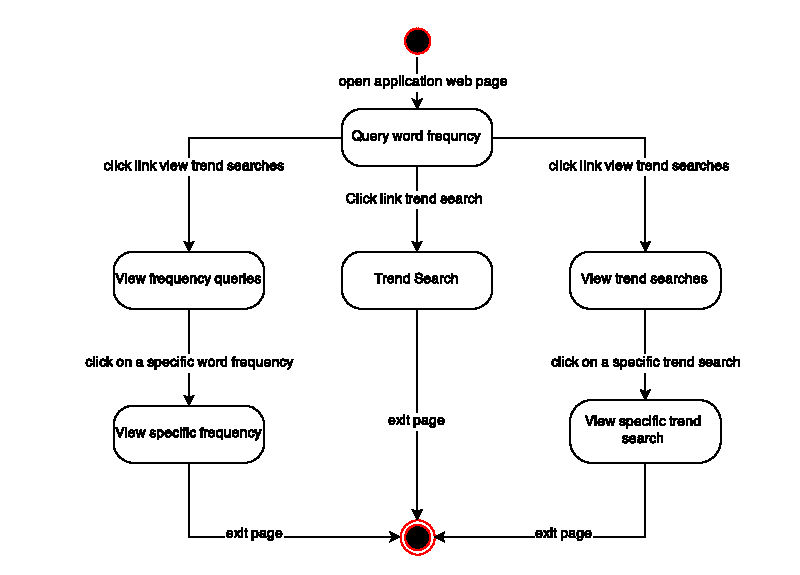
\includegraphics[width=15cm]{2_app_state_diagram}
\caption{Application state diagram}\label{app_state_diagram}
\end{figure}

In the following part of this chapter is described the most important class diagrams of \mbox{OpenMedia}. Most of them are related to the data mining part of the application. Information about the system components interaction is not enough for understanding the platform. The class diagrams deliver information under a higher level of granularity, hence the system becomes more easy to comprehend. Each step of the data gathering aspect of OpenMedia has a class diagram. It was mentioned that every custom fetcher should have it's own implementation but with a similar interface, it can be observed in \mbox{figure \ref{fetcher_class}}. Fetcher is the abstract class. It has a set of messages which are implemented by the custom implementations, such as UnimediaFetcher and TimpulFetcher.

\begin{figure}[!ht]
\centering
\vspace*{0.6cm}
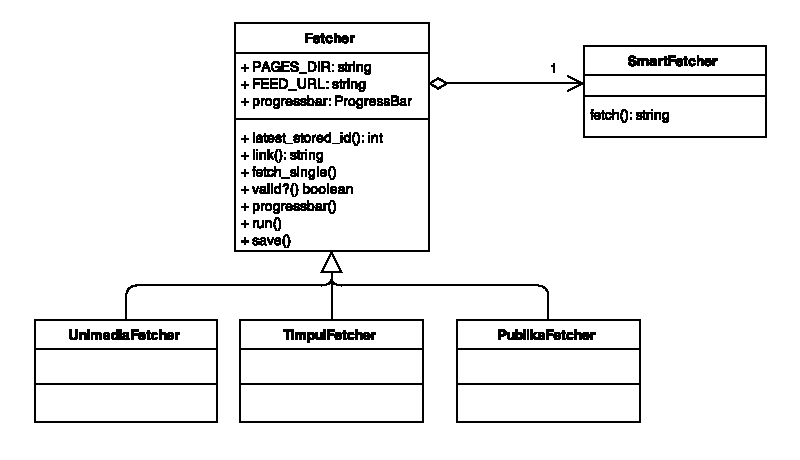
\includegraphics[width=16cm]{2_fetcher_class}
\caption{Fetching class diagram}\label{fetcher_class}
\end{figure}

The next class diagram, illustrated in \mbox{figure \ref{parser_class}}, depicts the parsing objects. The conceptual model is done in an analogical way. The defined abstract class has a set of predefined messages that denotes the possible actions needed to successfully get an article from file storage, parse it and save it to a database. The implementations of the abstract class are UnimediaParser and TimpulParser.

\begin{figure}[!h]
\centering
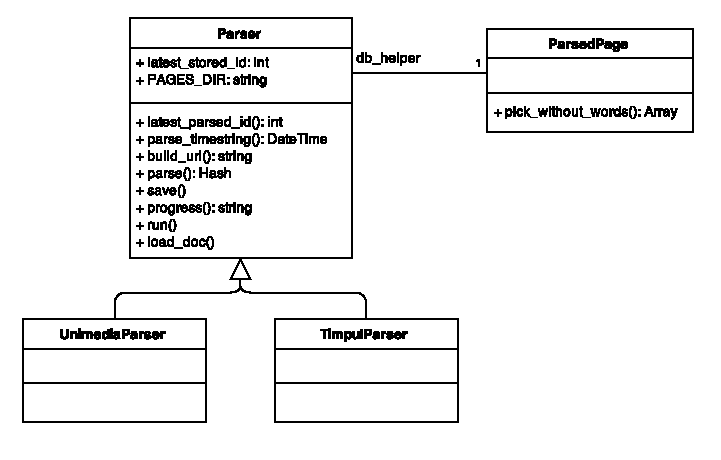
\includegraphics[width=16cm]{2_parser_class}
\caption{Parsing Class Diagrams}\label{parser_class}
\end{figure}

The last step of the data gathering platform is the natural language processing part. The class structure is much simpler, see \mbox{figure \ref{nlp_class}}. BatchRacaiFetcher class has association relationships with ParsedPage and Word model classes. Both are used for extracting data and saving it back. The main class aggregates RacaiBuilder. RacaiBuilder class is used for applying NLP actions on a given input. It is designed according to builder pattern. This offers to developers a high flexibility, the NLP actions can be performed in any sequence. The private methods encapsulate the communication via SOAP service. Under the hood the NLP actionso are request made to a web server.

\begin{figure}[!h]
\centering
\vspace*{0.6cm}
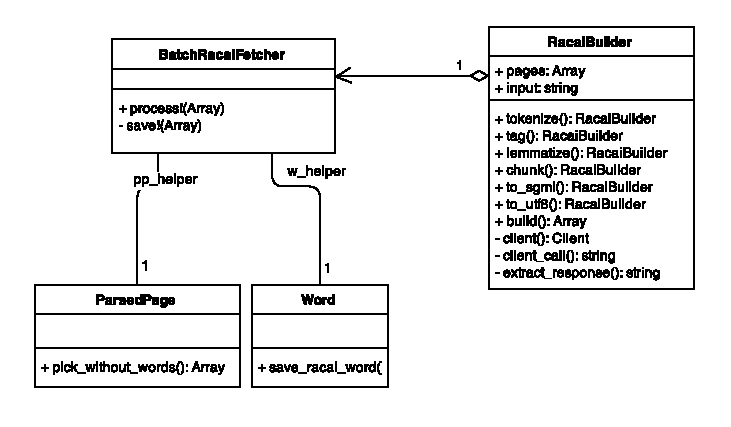
\includegraphics[width=16cm]{2_nlp_class}
\caption{NLP class diagram}\label{nlp_class}
\end{figure}

MongoDB models provide means to interact with the database. OpenMedia platform uses MongoDB as the primary database. The fields illustrated in the class diagram, \mbox{figure \ref{model_class}}, are mapped to the fields in database. All models inherit from Mongoid::Document class. Mongoid is the ORM used to create models in ruby. The inheritance marks the child class that it is used for database interactions. It also offers a set of messages that allows database operations. Such as finding an element, saving an element, different other type of queries.

\begin{figure}[!h]
\centering
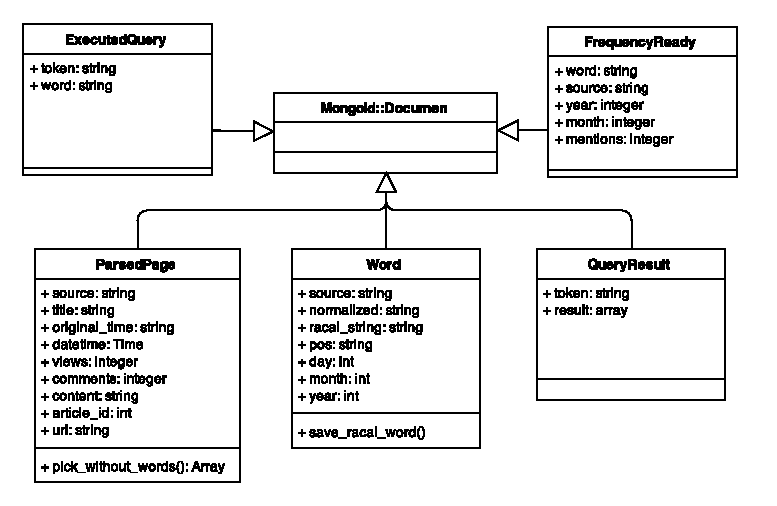
\includegraphics[width=16cm]{2_model_class}
\caption{MongoDB models class diagram}\label{model_class}
\end{figure}

The platform modules and their behavior were described until now. Another important part of the application is the set of libraries it uses and their purpose, depicted in \mbox{figure \ref{component_diagram}}. Because the project is divided in two parts there are two set of dependencies and libraries. The data mining part is a console applications, hence the set of required libraries is small. The essential library is rest\_client, used for requesting web pages and getting their content. Nokogiri is used for parsing HTML and extracting the necessary elements. Savon is a library for SOAP communications, needed for NLP processing. Mongoid is used for database communication, as it was discussed above. The client part of application requires more libraries because it consists from more logical components. Some gems (a ruby term for library) are shared between the logical components, for example Mongoid. Sinatra framework is used to build the web applications. The main goal is to handle client's HTTP requests. Faye library is used to host the websocket server. It is handy because it provides a higher level of functionality than a simple websocket. Haml gem aims to process the haml files for creating web page content. Haml is a dialect of HTML, simply put another markup language. Sidekiq is a library used for running asynchronous jobs. Redis is a dependency required by Sidekiq and it is used as a message queue system. D3 is a JavaScript library used for drawing plots and charts. This sums it up. Of cores there are also other dependency libraries.
\begin{figure}[!h]
\centering
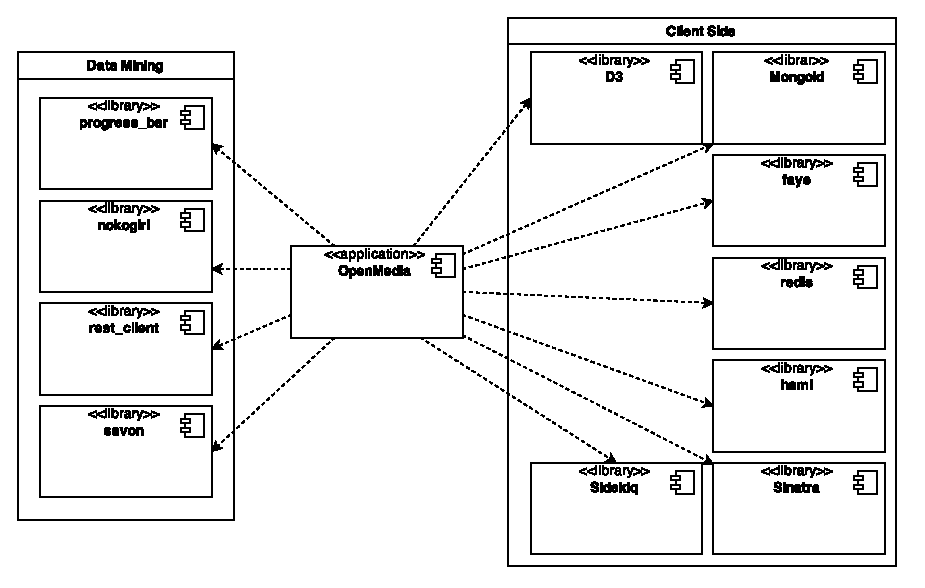
\includegraphics[width=16cm]{2_component_diagram}
\caption{Component diagram of OpenMedia}\label{component_diagram}
\end{figure}

The deployment diagram gives a good understanding of the whole system. OpenMedia platform has a complex structure and consist of more than a few modules, see \mbox{figure \ref{deployment}}. In order to launch the application, not every module needs to be up and running. Data mining application is a console ruby applications which only requires to run once in a while in order to keep the database content up to date. Moreover the NLP server is an external web service maintained by \emph{Institutul de Cercetare pentru Inteligență artificială Mihai Drăgănescu, Academia Română}. The diagram shows in details the complexity of OpenMedia platform. It also depicts the ways of communication between logical units of the application, concluding that some modules not only communicate with multiple entities, they also use different communication protocols. For instance Sinatra and Sidekiq servers communicates with three modules each, where the communication protocols are Mongoid API, Redis API, and the HTTP protocol. Another aspect is the operating systems used by every component. Linux is the main operating system for most of the modules. Regarding the client application, the operating system doesn't matter as long as it has installed a modern web browser. For Racai web service the operating system is unknown. This proves how powerful are the web services. A developer is not concerned about the internal infrastructure of the web service. As long as it complains a standard protocol a successful communication is achieved.

\begin{figure}[!ht]
\centering
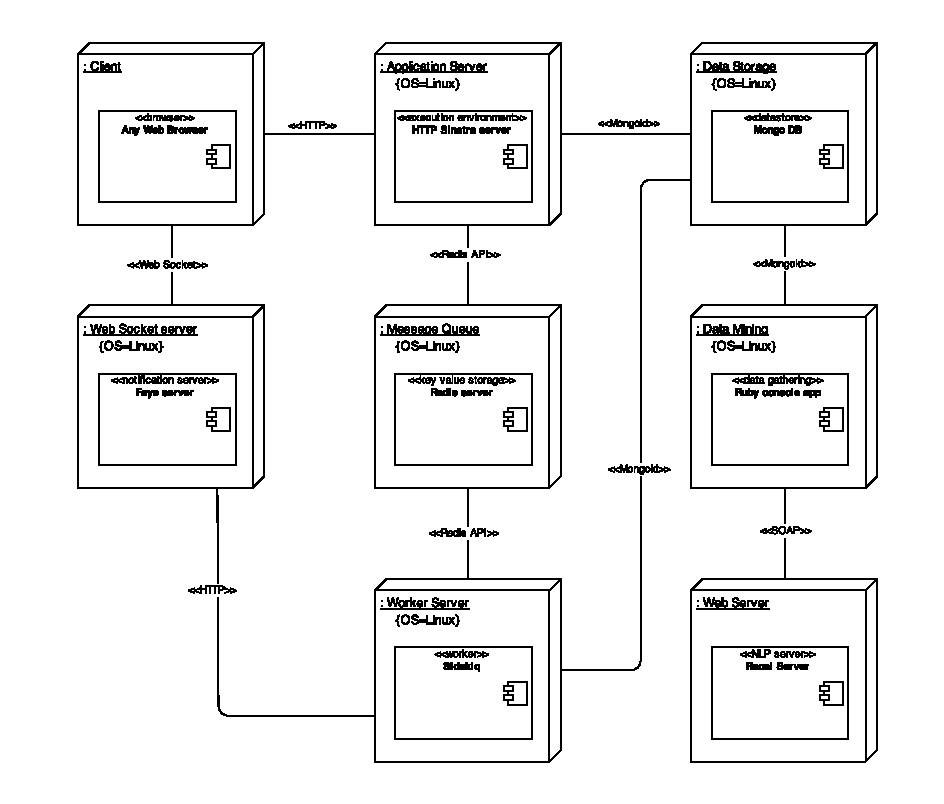
\includegraphics[width=18cm]{2_deployment}
\caption{OpenMedia deployment diagram}\label{deployment}
\end{figure}

Therefore the UML diagrams concentrate on the application prototype. They cover the most useful standard diagrams: use case diagrams, sequence diagrams, class diagrams, state diagrams, activity diagrams, components diagrams and deployment diagrams. All diagrams express the relationships, structural and behavioral aspects of the system. Modeling the application is for more reasons. The first and the obvious one, is to communicate the application architecture and its behavior. But the important aspect is, while modeling the platform the problem is understood better.

The implementation chapter focuses on the provided UML design, implements the classes and follows the use cases and sequence diagrams to define the flow of the application. The application components and dependencies will probably extend to a bigger degree. This concludes the UML description of the project, that aimed at presenting the most relevant aspect of the system and covering the general architecture of the application. The UML methodology offered a good documentation basis and a clear view on requirements of the software.